\section{Magdalena Janowska}
 Wyrażenie matematyczne:
\[\sinh=\frac{e^{x}-e^{-x}}{2}\]

 Zdjęcie: (Figure~\ref{fig:wykres})
\begin{figure} [htbp]
    \centering
    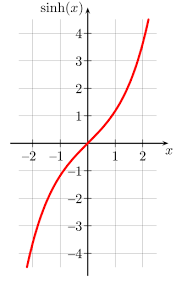
\includegraphics[scale=0.8]{pictures/wykres.png}
    \caption{Wykres funkcji sinh}
    \label{fig:wykres}
\end{figure}
 
 Lista numerowana:
\begin{enumerate}
    \item jeden
    \item dwa
    \item trzy
\end{enumerate}

 Lista nienumerowana:
\begin{itemize}
    \item jeden
    \item dwa
    \item trzy
\end{itemize}
 

 Tabela: ~\ref{tab:tabela}
\begin{table}[htbp]
    \centering
    \begin{tabular}{|c|c|c|c|c|}
\hline
\textbf{+}  & \textbf{1} & \textbf{2} & \textbf{3} & \textbf{4} \\ 
\hline
\textbf{1} & 2         & 3         & 4         & 5         \\ 
\hline
\textbf{2} & 3         & 4         & 5         & 6         \\ 
\hline
\textbf{3} & 4         & 5         & 6         & 7         \\ 
\hline
\textbf{4} & 5         & 6         & 7         & 8 \\ 
\hline
\end{tabular}
    \caption{Prosta tabela}
    \label{tab:tabela}
\end{table}


 Krótki tekst:\\
 
Lorem ipsum dolor sit amet, consectetur adipiscing elit. Nunc sed porta enim. Aliquam cursus vestibulum lacinia. \textbf{Curabitur suscipit, nisl id cursus auctor}, ex magna ullamcorper tortor, eget consectetur nisi nisi at sem.

In id risus dolor. Vestibulum fringilla vitae nisi nec scelerisque. Aliquam elementum molestie ligula, \emph{ in pretium velit hendrerit sit amet. Integer tempus erat ut velit faucibus}, malesuada mattis nibh dapibus. \textbf{Duis faucibus, est et sagittis accumsan,  \underline{lacus neque bibendum} nisi, nec rhoncus ligula nunc vitae urna.} 

    
    